\chapter{BOLUM ALTI BUYUK BASLIK}
\lipsum[1-2]
\acrlong{svm} , \acrlong{rf}, \acrlong{logreg}  ve \acrlong{cva}dır.

\section{Bölüm 6 alt başlık - bir}
\lipsum[3-4]
\acrfull{svm}  
\parencite{Hearst1998} 
\lipsum[6-8]
\acrshort{svm},  
$n$-\lipsum[11]

\begin{equation}
\overrightarrow{W}x_{i}+b = 0
\label{eq:ssss}%
\end{equation}

Eşitlik-\ref{eq:ssss}'de verilen $\overrightarrow{W}$ sd, $x_{i}$ olarak da supplyri, $b$ is değeri göstermektedir.

\lipsum[4]

\section{Bölüm 6 alt başlık - iki}
\lipsum[1-2]

\acrfull{rf}, 
\lipsum[8-10]


\begin{figure}[htp]
\centering
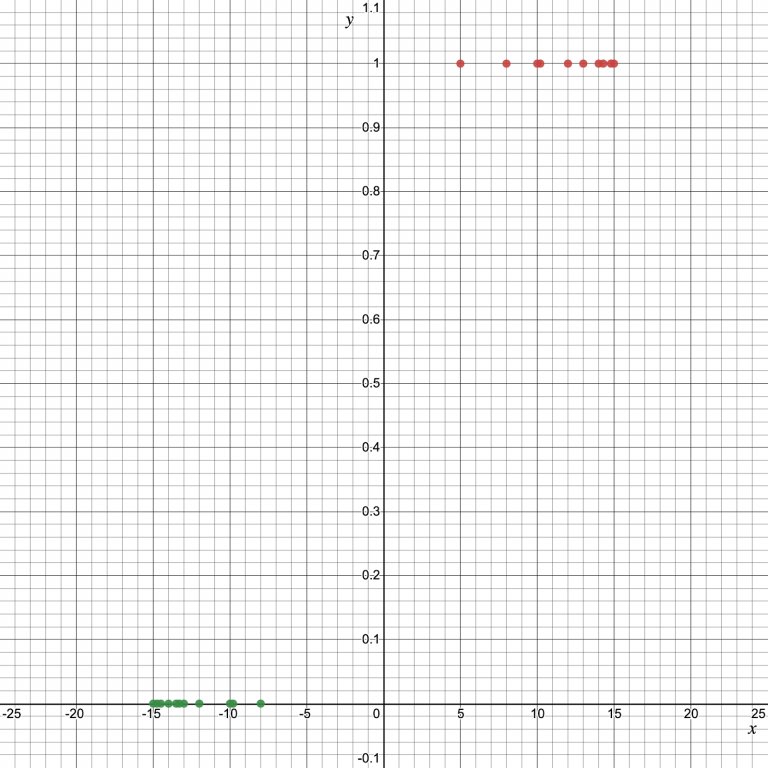
\includegraphics[width=0.69\textwidth]{gorseller/graph1.png}
\caption{yapnın yapısı}\label{fig:randomforest}
\end{figure}

\acrshort{rf}

\lipsum[3]

\addtocontents{toc}{~\hfill\underline{\textbf{Sayfa}}\vspace{0.3cm}\par} %% TODO: SAYFA YAZISI
% Cilt onay için reddedildikten sonra içerikteki ikinci kısma eklemek için dahil edildi.
\section{Bölüm 6 alt başlık - üç}
 \lipsum[1-2]



\acrfull{logreg} 
\lipsum[5]
Şekil-\ref{fig:ghsakjh}'de verilmiştir.  

\begin{figure}[htp]
\centering
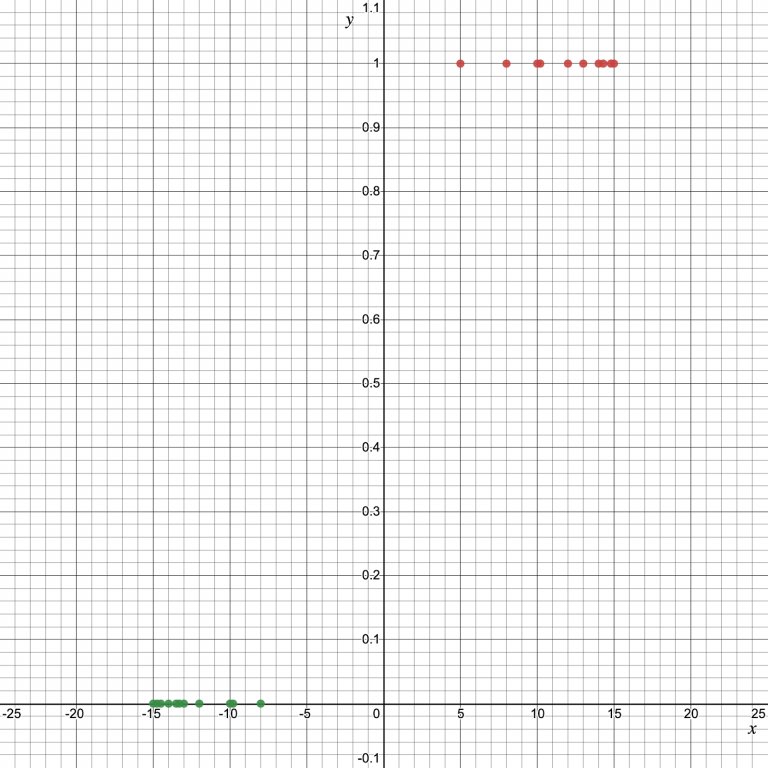
\includegraphics[width=0.45\textwidth]{gorseller/graph1.png}
\caption{Veri kümesindeki özniteliklerin düzlemdeki dağılımı}\label{fig:ghsakjh}
\end{figure}

 Eşitlik-\ref{eq:sadasfas}'dek

\begin{equation}
y = \frac{1}{(1+e^{-x})}
\label{eq:sadasfas}%
\end{equation}

\begin{figure}[htp]
\centering
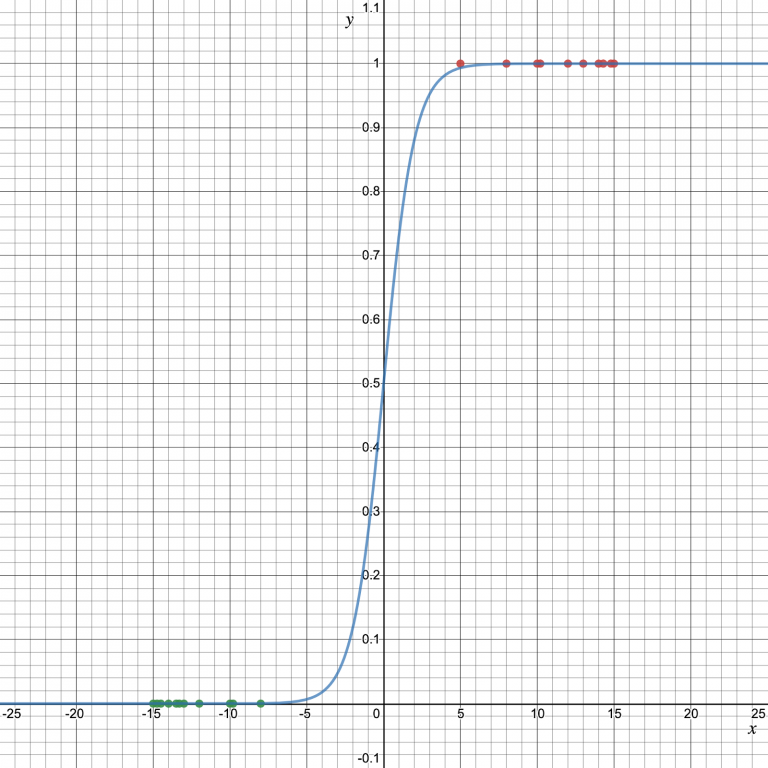
\includegraphics[width=0.45\textwidth]{gorseller/graph2.png}
\caption{Öznitelikler üzerine yerleştirilmiş sigmoid fonksiyonu}\label{fig:ghsakjh2}
\end{figure}

\lipsum[24]
\newpage
\section{Bölüm 6 alt başlık - dört}
% \lipsum[1-2]

\acrfull{cva}

\vspace{0.5cm}
\subsection{Bölüm 6 alt başlık - dört - alt başlık - 1}

\lipsum[10-12]

\subsection{Bölüm 6 alt başlık - dört - alt başlık - 2}

\lipsum[14-16]